\newcommand{\screenshotandformula}[3]{
	
	\begin{center}
		#3
		
		
		\hspace{2mm}	\includegraphics[width=0.4\textwidth]{images/#1}
		%	\hfill
		%	
\includegraphics[width=0.4\textwidth]{images/KW_muddychildren_redopened.png}
		
		#2
		
		
	\end{center}
	
}






\subsection{Open software}



\begin{frame}
	\frametitle{Open-source project}
	
	
	\begin{minipage}{6cm}
		\begin{center}
			
			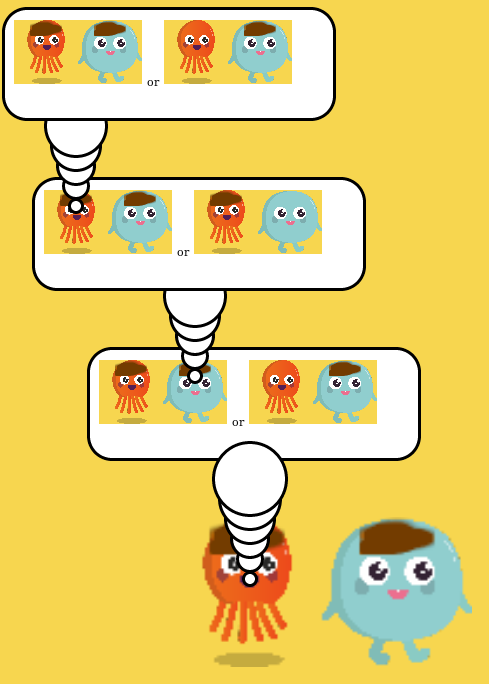
\includegraphics[width=3cm]{hintikka_world_screenshot.png}
			
			\url{http://hintikkasworld.irisa.fr/}
			
			~
			
			
			\url{https://gitlab.inria.fr/fschwarz/hintikkasworld}
			
			
			\mycitebiblio{demo IJCAI-ECAI 2018}
		\end{center}
	\end{minipage}
	\hfill
	\begin{minipage}{4cm}
		\begin{itemize}
			\item Web app
			\item Modular source code in Typescript
			
			\item Easy to add new examples
			\item Several contributors
			
			%Alexandre Niveau and Sébastien Gamblin (university of Caen) implemented BDDs in C and wasm
			
			%		\mycitebiblio{submission at demo IJCAI 2019}
			
			
		\end{itemize}
		
		
		
		\begin{block}{Please contribute}
			\begin{itemize}
				\item Coding
				\item Propose ideas and improvements
			\end{itemize}
		\end{block}
	\end{minipage}
\end{frame}







\subsection{Features}




%\begin{frame}
%\frametitle{Semantics of knowing something}
%\screenshotandformula{KW_muddychildren_redopened.png}{\coloragenta{Agent $a$} knows that \coloragentb{$b$} is dirty.}{\ok\hspace{1cm}\ok}
%\end{frame}

%
%\begin{frame}
%\frametitle{Possible worlds}
%\screenshotandformula{KW_muddychildren_redopened.png}{\coloragenta{Agent $a$} does not know that \coloragenta{he} is dirty.}{\hspace{1cm}\notok}
%\end{frame}





\newcommand{\loopabove}[1]{	\draw[->] (#1) edge [loop above] node {\agenta, \agentb} (#1);}
\tikzstyle{initialworld} = [initial left, initial text={}]
\tikzstyle{realevent} = [initial left, initial text={}]
\tikzstyle{realabove} = [initial above, initial text={}]
\tikzstyle{realworldarrowfromleft} = [initial left, initial text={}]



\newcommand{\enfantsalegd}{\begin{tikzpicture}[scale=0.3]
	\draw[fill=yellow!20] (0, 0) ellipse (1cm and 1cm);
	\draw[fill=blue!20] (0.3, 0.1) ellipse (.25cm and .25cm);
	\draw[fill=black] (0.4, 0.1) ellipse (.15cm and .15cm);
	\draw[red, line width=0.5mm] (0.2,-.3) edge[out=-90, in=180] (0.7, -0.7);
	\node at (0.4, 0.7) {
\includegraphics[scale=0.03]{images/tache.png}};
	\node at (-0.5, 0) {\tiny a};
	\end{tikzpicture}}

\newcommand{\enfantpropregd}{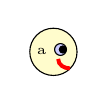
\begin{tikzpicture}[scale=0.3]
	\draw[fill=yellow!20] (0, 0) ellipse (1cm and 1cm);
	\draw[fill=blue!20] (0.3, 0.1) ellipse (.25cm and .25cm);
	\draw[fill=black] (0.4, 0.1) ellipse (.15cm and .15cm);
	\draw[red, line width=0.5mm] (0.2,-.3) edge[out=-90, in=180] (0.7, -0.7);
	\node at (-0.5, 0) {\tiny a};
	%	\node at (0.4, 0.7) {\includegraphics[scale=0.03]{images/tache.png}};
	\end{tikzpicture}}


\newcommand{\enfantsaledg}{\begin{tikzpicture}[scale=0.3]
	\draw[fill=yellow!20] (0, 0) ellipse (1cm and 1cm);
	\draw[fill=blue!20] (-0.3, 0.1) ellipse (.25cm and .25cm);
	\draw[fill=black] (-0.4, 0.1) ellipse (.15cm and .15cm);
	\draw[red, line width=0.5mm] (-0.2,-.3) edge[out=-90, in=0] (-0.7, -0.7);
	\node at (-0.4, 0.7) {
\includegraphics[scale=0.03]{images/tache.png}};
	\node at (0.5, 0) {\tiny b};
	\end{tikzpicture}}

\newcommand{\enfantpropredg}{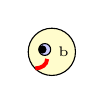
\begin{tikzpicture}[scale=0.3]
	\draw[fill=yellow!20] (0, 0) ellipse (1cm and 1cm);
	\draw[fill=blue!20] (-0.3, 0.1) ellipse (.25cm and .25cm);
	\draw[fill=black] (-0.4, 0.1) ellipse (.15cm and .15cm);
	\draw[red, line width=0.5mm] (-0.2,-.3) edge[out=-90, in=0] (-0.7, -0.7);
	\node at (0.5, 0) {\tiny b};
	%	\node at (0.4, 0.7) {\includegraphics[scale=0.03]{images/tache.png}};
	\end{tikzpicture}}


\newcommand{\mondereelenfantssales}[2]{\begin{tabular}{c}
		%	
\includegraphics[scale=0.08]{images/realworld.png} \\[-18mm]
		#1  #2 %\\[3mm]
		%	~
\end{tabular}}


\newcommand{\mondepossibleenfantssales}[2]{\begin{tabular}{c}
		%	
\includegraphics[scale=0.08]{images/possibleworld.png} \\[-18mm]
		#1  #2 % \\[3mm]
		%	~
\end{tabular}}



\newcommand{\exampleepistemicmodel}{\begin{tikzpicture}[yscale=0.7, xscale=0.45]
	\node[inner sep=0mm, realabove] (ss) at (0, 4) {\mondereelenfantssales\enfantsalegd\enfantsaledg};
	\node[inner sep=0mm]  (ps) at (5, 4) {\mondepossibleenfantssales\enfantpropregd\enfantsaledg};
	
	%
	%
	\node[inner sep=0mm]  (sp) at (0, 0) {\mondepossibleenfantssales\enfantsalegd\enfantpropredg};
	\node[inner sep=0mm]  (pp) at (5, 0) {\mondepossibleenfantssales\enfantpropregd\enfantpropredg};
	
	%	\onslide<2, 6>{\node[inner sep=0mm, fill=yellow] (ss) at (0, 4) {\mondereelenfantssales\enfantsalegd\enfantsaledg};}
	
	%	\onslide<3, 7>{\node[inner sep=0mm, fill=yellow]  (ps) at (5, 4) {\mondepossibleenfantssales\enfantpropregd\enfantsaledg};}
	
	%	\onslide<4, 8>{\node[inner sep=0mm, fill=yellow]  (sp) at (0, 0) {\mondepossibleenfantssales\enfantsalegd\enfantpropredg};}
	
	%	\onslide<5, 9>{\node[inner sep=0mm, fill=yellow]  (pp) at (5, 0) {\mondepossibleenfantssales\enfantpropregd\enfantpropredg};}
	
	\draw[<->] (ss) edge node[above] {\agenta} (ps);
	\draw[<->] (sp) edge node[above] {\agenta} (pp);
	\draw[<->] (ss) edge node[left] {\agentb} (sp);
	\draw[<->] (ps) edge node[right] {\agentb} (pp);
	\draw[->] (ss) edge [loop left,looseness=2] node {\agenta, \agentb} (ss);
	\draw[->] (sp) edge [loop left,looseness=2] node {\agenta, \agentb} (sp);
	\draw[->] (ps) edge [loop right,looseness=2] node {\agenta, \agentb} (ps);
	\draw[->] (pp) edge [loop right,looseness=2] node {\agenta, \agentb} (pp);
	\end{tikzpicture}}




\newcommand{\exampleeventmodel}{\begin{tikzpicture}
	\node[event, realabove] (e) at (0, 0) {\evenement \propositionaestsale - };
	\node[event]  (f) at (3,0) {\evenement {\vrai} - };
	
	%	\onslide<2-5>{\node[inner sep=0mm, fill=yellow] (e) at (0, 0) {\evenement \propositionaestsale - };}
	%	\onslide<6-9>{\node[inner sep=0mm, fill=yellow]  (f) at (4,0) {\evenementpossible {\formule{\vrai}} - };}
	
	\draw[->] (e) edge node[above] {\agentb} (f);
	\draw[->] (e) edge[loop left, looseness=2] node {\agenta} (e);
	\draw[->] (f) edge[loop right, looseness=2] node {\agenta, \agentb} (f);
	\end{tikzpicture}}



\newcommand{\examplefinalepistemicmodel}{\begin{tikzpicture}[yscale=0.7, xscale=0.6]
	%	\onslide<2->{
	\node[inner sep=0mm, realabove] (ssss) at (-6,7) {\mondereelenfantssales\enfantsalegd\enfantsaledg};
	\draw[->] (ssss) edge [loop left,looseness=2] node {\agenta} (ssss); %}
	
	
	%\onslide<2>{
	%		\node[inner sep=0mm, fill=yellow] (ssss) at (-6,7) {\mondereelenfantssales\enfantsalegd\enfantsaledg}; %}
	
	
	%			\onslide<4->{
	\node[inner sep=0mm] (sssp) at (-6,3) {\mondepossibleenfantssales\enfantsalegd\enfantpropredg};
	\draw[->] (sssp) edge [loop left,looseness=2] node {\agenta} (sssp); %}
	
	
	%\onslide<4>{
	%	\node[inner sep=0mm, fill=yellow] (sssp) at (-6,3) {\mondepossibleenfantssales\enfantsalegd\enfantpropredg}; %}
	
	
	%\onslide<6->{
	\node[inner ysep=1mm] (ss) at (0, 4) {\mondepossibleenfantssales\enfantsalegd\enfantsaledg};
	\draw[->] (ssss) edge node[above] {\agentb} (ss);
	\draw[->] (sssp) edge node[above, pos=0.7] {\agentb} (ss);
	\draw[->] (ss) edge [loop above,looseness=2] node {\agenta, \agentb} (ss);
	%}
	
	%\onslide<6>{
	%		\node[inner ysep=1mm, fill=yellow] (ss) at (0, 4) {\mondepossibleenfantssales\enfantsalegd\enfantsaledg}; %}
	
	%\onslide<7->{
	\node[inner sep=0mm]  (ps) at (5, 4) {\mondepossibleenfantssales\enfantpropregd\enfantsaledg};
	\draw[<->] (ss) edge node[above] {\agenta} (ps);
	\draw[->] (ps) edge [loop right,looseness=2] node {\agenta, \agentb} (ps);
	%}
	
	%\onslide<7>{
	%		\node[inner sep=0mm, fill=yellow]  (ps) at (5, 4) {\mondepossibleenfantssales\enfantpropregd\enfantsaledg};
	%}
	
	
	%
	%
	%\onslide<8->{
	\node[inner sep=0mm]  (sp) at (0, 0) {\mondepossibleenfantssales\enfantsalegd\enfantpropredg};
	\draw[->] (ssss) edge[out=-60] node[left, pos=0.8] {\agentb} (sp);
	\draw[->] (sssp) edge[out=-70, in=200] node[left] {\agentb} (sp);
	\draw[<->] (ss) edge node[left] {\agentb} (sp);
	\draw[->] (sp) edge [loop left,looseness=2] node {\agenta, \agentb} (sp);
	%	}
	
	
	%	\onslide<8>{
	%	\node[inner sep=0mm, fill=yellow]  (sp) at (0, 0) {\mondepossibleenfantssales\enfantsalegd\enfantpropredg};
	%}		
	
	%		\onslide<9->{
	\node[inner sep=0mm]  (pp) at (5, 0) {\mondepossibleenfantssales\enfantpropregd\enfantpropredg};
	\draw[<->] (sp) edge node[above] {\agenta} (pp);
	\draw[<->] (ps) edge node[right] {\agentb} (pp);
	\draw[->] (pp) edge [loop right,looseness=2] node {\agenta, \agentb} (pp);
	%}
	
	%		\onslide<9>{
	%			\node[inner sep=0mm, fill=yellow]  (pp) at (5, 0) {\mondepossibleenfantssales\enfantpropregd\enfantpropredg};
	%}
	
	
	
	
	
	
	\end{tikzpicture}}







%
%
%
%\begin{frame}
%	\frametitle{Epistemic states}
%	
%	\citeinslide{DitmarschvdHoekKooi}
%	
%	
%	Let $\atmset=\{p,p_1,\ldots\}$ be a countable set of atomic propositions.
%	
%	Let $\agtset=\{\agenta,\agentb,\agentc,\ldots\}$ be a finite set of agents.
%	
%	\vfill
%	\begin{definition} 
%		
%		\label{def-epsmodel}
%		
%		An \alert{epistemic model} $\kripkemodel=(\setworlds,(\relworldsa)_{a\in\agtset},\valuationfunction)$ is a tuple  where: 
%		
%		\begin{itemize}
%			
%			\item $\setworlds=\{\aworld,\aworldb,\ldots\}$ is a non-empty set of possible \emph{worlds};
%			\medskip
%			\item $\relworldsa\subseteq \setworlds\times \setworlds$
%			is an
%			\emph{accessibility relation} for agent $a$;
%			\medskip
%			\item $\valuationfunction:\setworlds\rightarrow 2^\atmset$ is a \emph{valuation function}.
%			
%		\end{itemize}
%		
%	\end{definition}
%	
%	\vfill
%	
%	
%	A pair $(\kripkemodel,w)$ is called a \alert{epistemic state},
%	where $w$ represents the actual world.
%\end{frame}
%
%

%
%
%\begin{frame}
%	\frametitle{Example}
%	
%	\begin{tikzpicture}[scale=0.9]
%		\node {\exampleepistemicmodel};
%		\node at (-2, 2) {$w$};
%		\node at (2, 2) {$u$};
%		\node at (-2, -2.5) {$v$};
%		\node at (2, -2.5) {$s$};
%	\end{tikzpicture}
%
%	\vfill
%	
%	\small
%	\begin{itemize}
%		\item $W = \set{w, u, v, s}$;
%		\item $R_a = \set{(w, w), (w, u), (u, w), (u, u), (v, v), (v, s), (s, v), (s, s)}$;
%		\item $R_b = \set{(w, w), (w, v), (v, w), (v, v), (u, u), (u, s), (s, u), (s, s)}$;
%		\item $V(w) = \set{\propositionaestsale, \propositionbestsale}$;
%		\item $V(u) = \set{\propositionbestsale}$;
%		\item $V(v) = \set{\propositionaestsale}$;
%		\item $V(s) = \emptyset$.
%	\end{itemize}
%	
%\end{frame}

\newcommand{\loopleft}[1]{\draw[->] (#1) edge[loop, loop left, looseness=1] node {\agenta, \agentb, \agentc} (#1);}
\newcommand{\loopright}[1]{\draw[->] (#1) edge[loop, loop right, looseness=1] node {\agenta, \agentb, \agentc} (#1);}
\newcommand{ \propositionpossedecarte}[2]{\propositiontxt{#1 possède #2}}














\tikzstyle{bullecommunaute} = [fill=green!50!white, circle, minimum height=1cm]


\begin{frame}
\frametitle{Many examples from different communities}

\begin{center}
\begin{tikzpicture}
\node[bullecommunaute] {~~~~~~~~~~~~~~~~~~~~~~~~~~~~~~~~~~};
\node[bullecommunaute] at (-0.7, 0.5) {Logic};
\node[bullecommunaute] at (0.7, 0.5) {Verification};
\node[bullecommunaute] at (0, -0.5) {AI};
\node at (-4, 0) {Robotics};
\node at (-2, 2) {Psychology};
\node at (0, 3) {Distributed systems};
\node at (2, 2) {Cryptography};
\node at (3, 0) {Games};
\node at (0, -3) {Philosophy};
\pause
\node at (-4, 2) {
\includegraphics[height=1cm]{images/HW_example_sally_and_ann.png}};
\node at (4, 2.8) {
\includegraphics[height=1cm]{images/HW_example_dining_cryptographers_problem.png}};
\node at (4, -1) {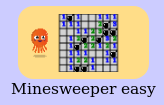
\includegraphics[height=1cm]{images/HW_example_minesweeper.png}};
\node at (-4, -2) {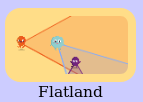
\includegraphics[height=1cm]{images/HW_example_flatland.png}};
\end{tikzpicture}
\end{center}



\end{frame}






\begin{frame}
	\frametitle{Many examples}
	\begin{center}
		
\includegraphics[height=6cm]{images/examples.png}
	\end{center}
\end{frame}





%
%
%\begin{frame}
%\frametitle{Dual operators}
%
%%The
%%semantics of $\languageEL$ is defined as follows:
%
%
%\begin{center}
%		\screenshotandformula{KW_muddychildren_redopened.png}{Agent $a$ knows that $b$ is dirty.}{\ok\hspace{1cm}\ok}
% \ok\hspace{2.5cm}
%	
%	
\includegraphics[width=0.4\textwidth]{images/KW_muddychildren_redopened.png}
%	
%	agent $a$ considers possible that $b$ is dirty
%	
%
%	$\modelM, w \models \lknowpos a \propositionaestsale$
%\end{center}
%
%\end{frame}











